\documentclass{article}
\usepackage[utf8]{inputenc}
\usepackage[spanish]{babel}
\usepackage{listings}
\usepackage{graphicx}
\graphicspath{ {images/} }
\usepackage{cite}

\begin{document}

\begin{titlepage}
    \begin{center}
        \vspace*{1cm}
            
        \Huge
        \textbf{Nociones de la memoria del computador}
            
        \vspace{0.5cm}
        \LARGE
        
        
            
        \vspace{1.5cm}
            
        \textbf{Johan Fernando Mora Ramirez}
        
         \vspace{1.5cm}
         \begin{figure}[h]
        
\includegraphics[width=4cm]{EscudoUdea.jpg}
        \centering
       
        \label{fig:EscudoUdea}
        \end{figure}
            
        \vfill
            
        \vspace{0.8cm}
            
        \Large
        Despartamento de Ingeniería Electrónica y Telecomunicaciones\\
        Universidad de Antioquia\\
        Medellín\\
        Septiembre de 2020
            
    \end{center}
\end{titlepage}

\tableofcontents
\newpage
\section{Sección introductoria}\label{intro}
Al momento de llevar a cabo la elaboración de un proyecto ya sea en el ámbito de la programación o en cualquier otro, algo de suma relevancia es la optimización de recursos empleados en el desarrollo de este, consecuentemente se hace necesario tener un conocimiento previo al respecto de elementos fundamentales como lo es la memoria de un computador, su funcionamiento, capacidades, variedades y usos específicos.


\section{Sección de contenido} \label{contenido}
En esta sección se lleva a cabo la solución de los diferentes interrogantes respecto a la memoria del computador propuestos por el docente del curso.

\subsection{Defina que es la memoria del computador.}

La memoria del computador es uno de sus componentes más importantes, pues en este dispositivo donde se llevan a cabo los procesos de almacenamiento y procesamiento de datos e instrucciones generados por los microprocesadores del computador. Dependiendo de su velocidad y capacidad de almacenamiento a las memorias se le asignan labores específicas, ya sean almacenar datos de manera permanente o cargar en estas solo la información requerida en cada instante de tiempo, no obstante y pese a que cada uno de los tipos de memoria de un computador es indispensable para su correcto funcionamiento, el tipo de memoria RAM es el más importante debido a que es en esta en la que se almacena y procesa momentáneamente toda la información requerida por los microprocesadores y sus respectivas instrucciones.

\subsection{Mencione los tipos de memoria que conoce y haga una pequeña descripción de cada tipo.}

\textbf{Memoria RAM:} (Random Access Memory - Memoria de Acceso Aleatorio). Figura (\ref{fig:Memoria_RAM}). 
La memoria RAM como se mencionó anteriormente se puede considerar la más importante de un computador, Su nombre proviene del hecho de que puede grabarse o recuperarse información de ella sin necesidad de un orden secuencial, en esta residen programas y datos sobre la que se pueden efectuar operaciones de lectura y escritura, se ejecuta la mayor parte del software (el sistema operativo, software de aplicación, etc.) y es una forma de memoria temporal, que al apagar o reiniciar el sistema vuelve a estar en blanco.\cite{Consepto.de}




\vspace{0.5cm}


\textbf{Memoria ROM:} (Read Only Memory - Memoria de Sólo Lectura). Figura (\ref{fig:Memoria_ROM}).Evita la sobreescritura los datos contenidos en ella, este tipo de memoria se emplean para almacenar información de configuración del sistema, programas de arranque o inicio, soporte físico y otros programas que no precisan de actualización constante.\cite{Definición ABC}

\vspace{0.5cm}

\textbf{Memoria Cache:} Figura  (\ref{fig:Memoria_Cache}).Se utiliza para almacenar y procesar los datos que el microprocesador utiliza más frecuentemente, esto porque pese a su escasa capacidad de almacenamiento tiene una velocidad muy superior a la memoria RAM, se encuentra dentro del microprocesador y se divide en tres niveles L1, L2 y L3. La memoria Cache L1 es la más rápida seguida por la L2 que es un poco más lenta, pero con mayor capacidad de almacenamiento, ambas están incorporadas dentro del microprocesador y por último esta la L3 que aun siendo más lenta de todas tiene la mayor capacidad de las 3.

\vspace{0.5cm}

\textbf{Disco Duro:} Figura (\ref{fig:Disco_Duro}). Un disco duro, también denominado disco rígido, es un dispositivo de almacenamiento de datos no volátil pues los contenidos almacenados no se pierden, aunque no se encuentre energizado, este emplea un sistema de grabación magnético para guardar los datos digitales y si bien este es el tipo de memoria con mayor capacidad de almacenamiento del computador, también es cierto que es el más lento.

\vspace{0.5cm}

\textbf{Imagenes:}

\begin{figure}[h]
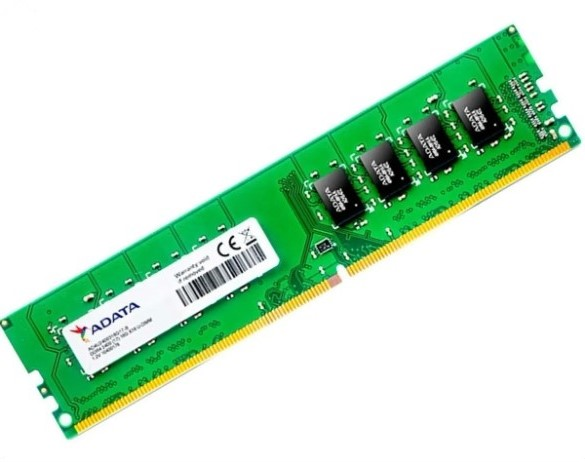
\includegraphics[width=3.2cm]{Memoria_RAM.jpg}
\centering
\caption{Memoria RAM}
\label{fig:Memoria_RAM}
\end{figure}

\begin{figure}[h]
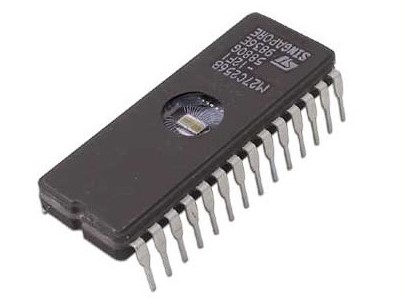
\includegraphics[width=3.2cm]{Memoria_ROM.jpg}
\centering
\caption{Memoria ROM}
\label{fig:Memoria_ROM}
\end{figure}

\begin{figure}[h]
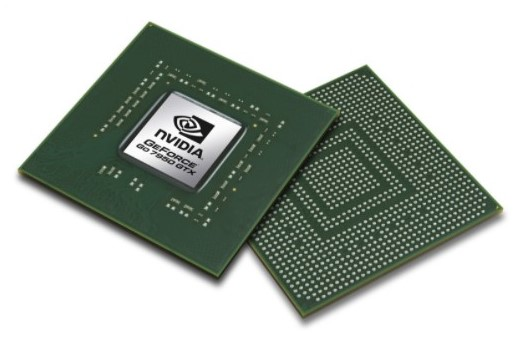
\includegraphics[width=3.2cm]{Memoria_Cache.jpg}
\centering
\caption{Memoria Cache}
\label{fig:Memoria_Cache}
\end{figure}

\begin{figure}[h]
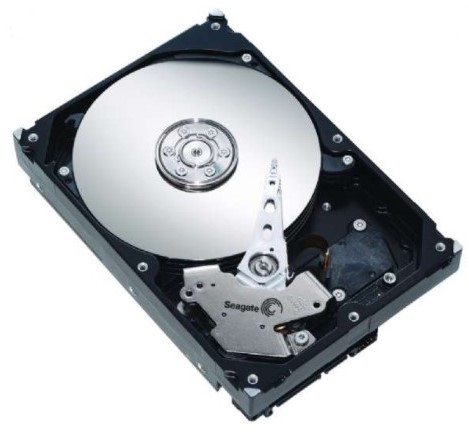
\includegraphics[width=3.2cm]{Disco_Duro.jpg}
\centering
\caption{Disco Duro}
\label{fig:Disco_Duro}
\end{figure}

\subsection{Describa la manera como se gestiona la memoria en un computador.}

Al momento de encender el computador el microprocesador procede a leer las instrucciones de la memoria ROM la cual le ordena que se hagan una serie de chequeos para comprobar que todos los componentes funcionen adecuadamente, eventualmente la BIOS provee información al respecto de los dispositivos de almacenamiento y en cual se encuentra el sistema operativo que posteriormente es copiado del disco duro y cargado en la memoria RAM durante el tiempo que el equipo este encendido, las  instrucciones dadas por el usuario a cada instante son interpretadas y ejecutadas por el procesador para luego ser eliminadas de la memoria, si se desea editar algún tipo de información esta se obtiene del disco duro y se ubica en la memoria RAM para ser procesada y una vez editada se guarda nuevamente en el disco duro mientras es eliminada de la RAM, al momento de ejecutar un software de igual manera este es copiado del disco duro en la RAM durante el tiempo que permanezca en ejecución, una vez el computador se apague el disco duro conservará toda la información contenida en el mientras que la memoria RAM quedara completamente en blanco.

\subsection{¿Qué hace que una memoria sea más rápida que otra? ¿Por qué esto es importante?}

Los discos duros emplean sistemas de grabación magnética y su funcionamiento se basa en un trabajo mecánico en el cual uno o varios discos rígidos unidos por un mismo eje giran rápidamente en torno a este, mientras un cabezal de lectura/escritura se encuentra sobre cada uno de ellos.
Las memorias de tipo DRAM funciona a partir de celdas de memoria que contienen transistores y capacitores microscópicos que se cargan y descargan en representación de bits que constantemente son cargados por un controlador e interpretados de manera electrónica en periodos de nanosegundos.
En el tipo de memoria SRAM cada celda de bit está compuesta por cuatro o seis transistores y algunos circuitos; logrando que no sea necesario refrescar la información recargando las celdas constantemente como sucede con la memoria dinámica (DRAM).

los tipos de memoria mencionados anteriormente  difieren notablemente entre sí, tanto en su capacidad de almacenamiento como en su velocidad y se puede deducir que dichas diferencias se deben esencialmente a su diseño y arquitectura, pues es esta la que define el funcionamiento particular de la memoria en cada caso, es decir si se compara la velocidad con la que gira un disco mecánico y la velocidad a la que se mueven los electrones en un circuito hay una diferencia abismal, del mismo modo que si se compara un sistema que continuamente debe ser actualizado por un controlador y uno que no, también se puede apreciar una diferencia notoria en cuanto a la eficiencia de ambos.

\vspace{0.5cm}

La importancia de que existan diferentes tipos de memoria con diferentes funcionamiento, cualidades y defectos radica en el hecho que un dispositivo tan complejo como lo es el computador necesita diferentes soluciones para los múltiples retos que supone lograr un óptimo funcionamiento de este con el menor coste posible, de esta manera dependiendo de la necesidad particular que se tenga es posible implementar el uso de uno u otro tipo de memoria entre la variedad existente.


\section{Conclusiones} \label{contenido}

Existe una gran variedad de memorias con características especificas (velocidad, almacenamiento, tamaño, etc.) que dependen esencialmente de su respectiva arquitectura y el principio de su funcionamiento.

Si bien los computadores cuentan con cierta cantidad de memorias que son indispensables para su correcto funcionamiento, la memoria RAM es la más importante de todas pues es la que permite tener a disposición del microprocesador la información que este necesita en cada instante y de una manera muy eficiente.

Como ingeniero es indispensable poder brindar soluciones optimas y eficientes a los diferentes retos propuestos, esto implica saber administrar correctamente los recursos que se tengan disposición de tal manera que representen el menos coste posible, en este caso la memoria resulta ser un recurso muy valioso que debe ser administrado de la manera más optima.

\bibliographystyle{IEEEtran}
\bibliography{references}

\end{document}
